\chapter{How we tested it: the evaluation design}
\label{ch:eval}

\section{The ground rules: what makes a test fair}
\begin{simplebox}
A fair test has four rules. (1) \textbf{The answer key is hidden.} The tool must not be able to peek at what was actually broken. (2) \textbf{The faults are physical.} We really kill, pause and starve containers, we do not just edit numbers. (3) \textbf{The test set is separate from the tuning set.} You do not grade a student on the questions you taught them with. (4) \textbf{Report the whole picture.} Include the weak results, with error bars.

We followed all four, within the limits we describe honestly later.
\end{simplebox}

\section{The two real systems we built}
\begin{simplebox}
We did not use someone else's demo app. We built two realistic systems, each in its own repository, each on its own cloud machine:

\begin{itemize}
\item \textbf{ShopFlow}: an online shop checkout with 13 services (a gateway, catalogue, cart, inventory, payments, orders, a notification consumer, a pretend third-party payment provider, plus databases, caches and a message bus).
\item \textbf{LedgerLine}: a bank-transfer system with 12 services (an edge, accounts, transfers, fraud screening, FX rates, a double-entry ledger, a statements worker, a pretend third-party FX provider, plus databases and a message bus).
\end{itemize}

Each comes with a monitoring stack (Prometheus, Grafana, Loki), an always-on traffic generator that mimics visitors with a daily wave, bursts and flash crowds, and a \emph{Fault Lab}: the fault injector.
\end{simplebox}

\begin{techbox}
Each bench runs on an EC2 \code{c7i-flex.large} host (2 vCPUs, 4\,GiB; about 0.6\,GiB of containers) in \code{ap-south-1}. The code of both is deliberately correct and defensive: every failure comes from configuration, data volume, sizing, topology or a third party, and every scripted scenario ships with a machine-readable ground truth (true root cause, what a monitor should and should not see, the fix). Monitoring is a \emph{separate Compose project}, so the application project stays exactly what a mapper should discover. A ``dashboard viewer'' container queries Grafana every few seconds, as a person watching would, so those links are live.
\end{techbox}

\begin{figure}[H]
\centering
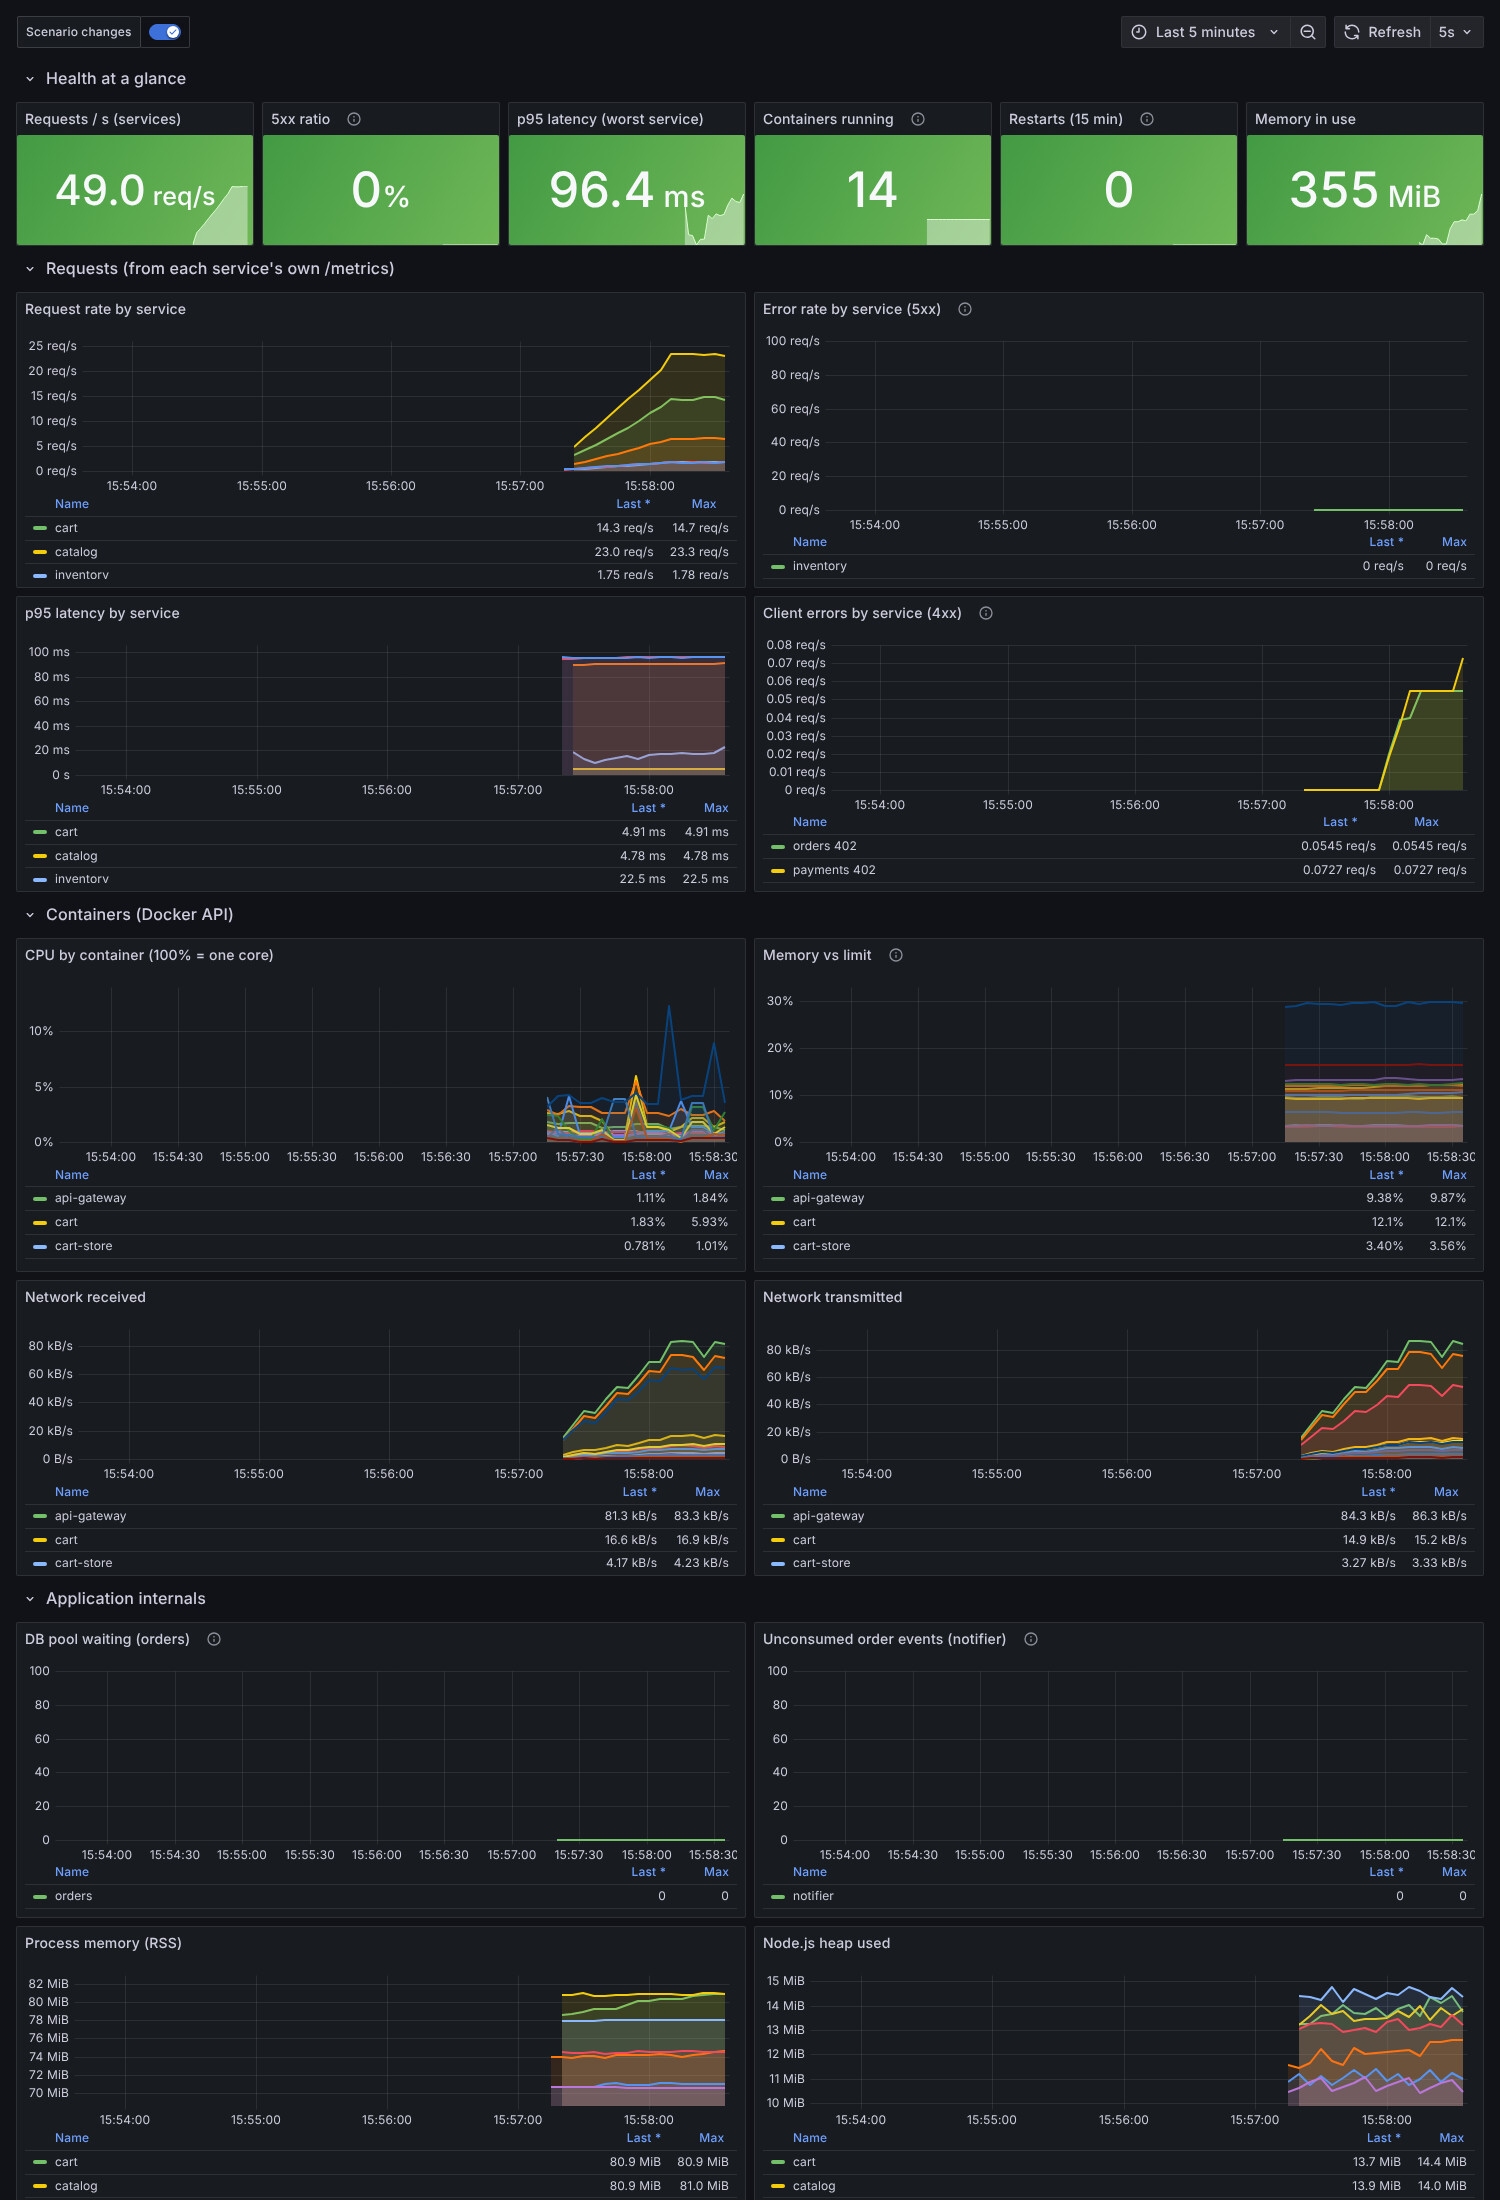
\includegraphics[width=0.5\textwidth]{grafana_shopflow.jpg}\hfill
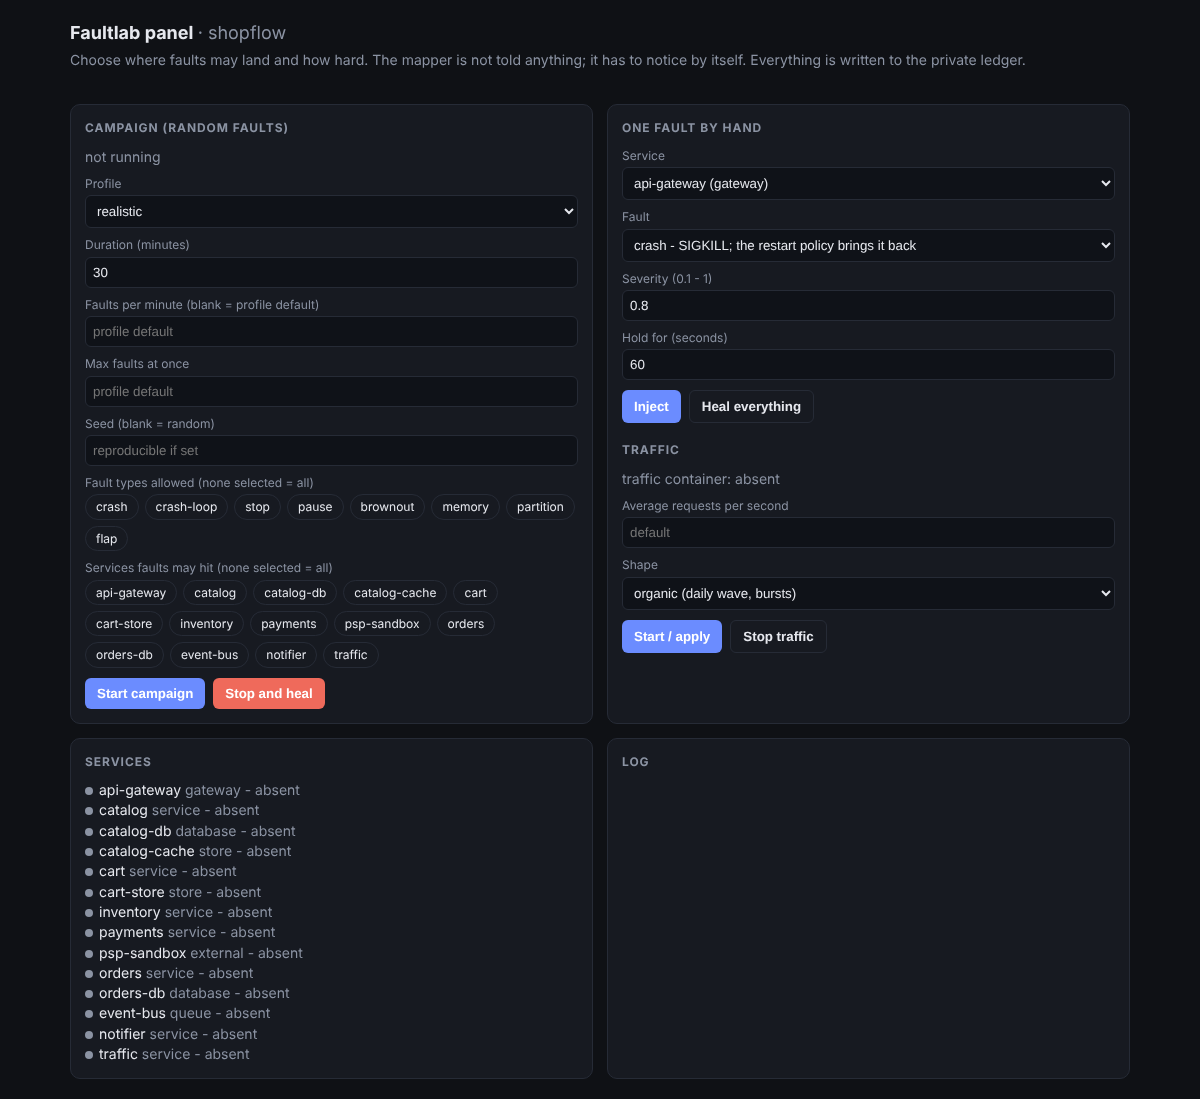
\includegraphics[width=0.46\textwidth]{faultlab_shopflow.png}
\caption{Left: the ShopFlow Grafana dashboard. Right: the Fault Lab control page.}
\end{figure}

\section{The Fault Lab: three properties}
\begin{simplebox}
\textbf{Blind.} The mapper is never told what is injected. The injector writes every fault into a private notebook (a ``ledger'') that nobody reads until scoring. \textbf{Physical.} Faults act on containers: kill, repeated kills, stop, pause, resource limits that slow a service, network detach, repeated pause-and-release. \textbf{Reproducible.} A campaign draws faults at random from a Poisson process with a profile, rate and seed; the same seed gives the same campaign.
\end{simplebox}

\begin{techbox}
Faults arrive by a non-homogeneous Poisson process whose rate follows the load, each with a class, a role-weighted target, a heavy-tailed duration and a severity; with some probability a follower is spawned in the target's one-hop neighbourhood, so incidents overlap. The ledger records, per fault, the true root cause and the services structurally able to be affected. The control page runs on the bench host, listens on localhost only and requires a header only the page itself sets, so another site open in the same browser cannot drive it. The two real systems contribute 62 faults over seven classes (crash, stop, brownout, memory, crash-loop, pause, flap).
\end{techbox}

\section{Four kinds of data}
\begin{center}
\small
\begin{tabularx}{\textwidth}{>{\raggedright\arraybackslash}p{2.7cm}>{\raggedright\arraybackslash}p{2.7cm}>{\raggedright\arraybackslash}X}
\toprule
\textbf{Data} & \textbf{Size} & \textbf{What it is for}\\
\midrule
Real recorded campaigns & 62 faults, 217 min each, both benches & The main result on real systems.\\
Live campaigns & 84 faults (21 per run; both benches; auto-restart on and off) & Check the mapper against a system it cannot see into, and test auto-restart.\\
Synthetic held-out & 178 faults, 16 topologies, seed 2, scored once & Enlarge the sample; test generalisation to topologies not tuned on.\\
Synthetic tuning & 170 faults, 16 campaigns, seed 1 & Choose settings; never used for reported numbers.\\
Workload recordings (no fault) & 62 min organic on/off; 72 min stepped $2,8,2,0,20,2$ visitors & Count false alarms when only the load changes; every alarm is false by construction.\\
\bottomrule
\end{tabularx}
\end{center}

\begin{warnbox}
The 62 real faults are not tuned on a held-out real system. Say ``the synthetic numbers come from a split scored once; the real numbers are optimistic by an amount we cannot measure''. Also: the workload recordings come from traffic generators, not real users.
\end{warnbox}

\section{The measures}
\begin{simplebox}
We needed measures that match how an operator experiences the tool, so we did not use a simple ``percentage of readings classified correctly''. We use event-level measures.

\begin{itemize}
\item \textbf{Detected}: an alarm names a truly involved service while the fault is active.
\item \textbf{Caught and named (C+N)}: detected, \emph{and} the true root cause was ranked first. This is the headline number.
\item \textbf{A@1, A@3}: among detected faults, how often the truth was first, or in the top three.
\item \textbf{False-alarm episodes per fault-free hour (FA/h)}: alarms outside every fault window, with one unbroken alarm counting as one episode.
\item \textbf{Alarm time}: the share of fault-free time the engine spent in alarm.
\item \textbf{Detection delay}: seconds from fault onset to the first alarm.
\end{itemize}

Why two false-alarm measures? One unbroken alarm counts as one episode, so an engine can look good on episodes while alarming almost all the time. Alarm time exposes that. An earlier version of our own detector had a low episode rate and 86\% alarm time on the real systems; after the refinements it was 5\%.
\end{simplebox}

\begin{techbox}
Point-wise scoring with a window adjustment (credit a whole event if any point is flagged) rewards an engine that flags one point of a long fault; that is not how an operator experiences an alarm. Warm-up (the first five minutes of each run) is excluded from false-alarm and ROC counts. Intervals are 95\% percentile bootstrap intervals over faults; comparisons between engines are \emph{paired} bootstrap differences over the same faults with two-sided $p$ values. Overlapping faults within a run are not independent, so intervals are, if anything, optimistic. With 62 real faults a difference below about 8--10 points cannot be resolved.
\end{techbox}

\section{What a bootstrap confidence interval means (so you can explain it)}
\begin{simplebox}
We have 62 faults and the tool caught and named 44 of them (71\%). Is the true rate 71\%? Not exactly: with a different 62 faults we would have got a slightly different number. To see how much the number wobbles, we pretend our 62 faults are the whole world, draw 62 faults \emph{with replacement} many times, compute the rate each time, and read off the middle 95\% of those rates. That range is the confidence interval. For 71\% on 62 faults it is about $[60, 81]$.
\end{simplebox}

\begin{examplebox}[A paired comparison in one paragraph]
To ask ``is Hybrid better than Rules?'' we do not compare two separate intervals. We look at the \emph{same} 62 faults under both engines. For each fault, record whether Hybrid got it and Rules did not (+1), the reverse ($-1$) or both/neither (0). Average these differences, and bootstrap the average. The result is $+8.1$ points, 95\% interval $[-1.6,+17.7]$. The interval includes zero, so we cannot rule out ``no difference'', and the $p$ value is 0.117 (not below 0.05).
\end{examplebox}

\section{Two measurement bugs, which we found and fixed}
\begin{simplebox}
\textbf{Bug 1: the notebook was half-read.} Each recorded run held two fault campaigns, and both numbered their faults from one. Our reader kept only the second, so for every engine 14 of 31 faults per system were hidden, and the outages of the hidden faults were counted as \emph{false alarms}. Every number in the report uses all 62 faults now, and a test guards the reader.

\textbf{Bug 2: the replay threw away the quiet parts.} The tool that replays recorded runs skipped a reading when it matched the previous one. An idle service reports the same zeros again and again, so the replay deleted exactly the idle stretches. That is why the old forest looked fine in our benchmarks when traffic stopped; the live system does not skip readings. We fixed the replay and recomputed every number that depended on it.
\end{simplebox}

\begin{saybox}
``Both bugs made the engines look \emph{better} than they were, and we found them ourselves. That is why we trust the numbers in the report: they are what is left after we tried to break our own evaluation.''
\end{saybox}
